

hhhjhlkjgkjh

- teoria de llum (laser + aigua)
- estructura de la fibra, gruxut
- comunicarse atraves de la llum

- usuarios que utilizan opticas
- fabriques mundials
- processos de fer
- el preu
- 1841 fanshe
- cristal

\subsection*{Introducció}
\addcontentsline{toc}{subsection}{Introducció}
La comunicació amb llum visible (coneguda com a VLC, acrònim en anglès de "visible light communication") és un mitjà transmissor de dades que utilitza la llum entre 400 i 800 THz (780-375 nm). VLC és un subconjunt de tecnologies de comunicacions òptiques sense fil.

Altres subconjunts són:
\begin{itemize}
    \item Infraroig (IR): Encara que no és visible per a l'ull humà, la llum infraroja s'utilitza en diverses tecnologies sense fil, com ara els controls remots, els dispositius de comunicació a curta distància i les transmissions de dades sense fil en alguns contextos.
    \item Comunicació Òptica d'Espai Lliure (FSO): Aquesta tecnologia utilitza feixos de llum làser per a la transmissió de dades sense cables a través de l'espai lliure, com ara entre dos edificis. És especialment útil en línies de vista directa sense obstruccions.
    \item Comunicació Òptica Inalàmbrica (OWC): Aquesta tecnologia inclou diverses formes de transmissió de dades sense fil a través de llum òptica, incloent l'ús de làsers i LED.
    \item Comunicació Òptica en Entorns Controlats: En alguns entorns, com ara entorns d'oficines o fàbriques, es poden utilitzar sistemes d'òptica sense fil per a la transmissió de dades en lloc de les tecnologies tradicionals sense fil.
\end{itemize}

cada tecnologia té les seves pròpies aplicacions, avantatges i desavantatges. La selecció de la tecnologia òptica sense fil adequada depèn dels requisits específics de l'aplicació i les condicions de l'entorn.

\begin{center}
    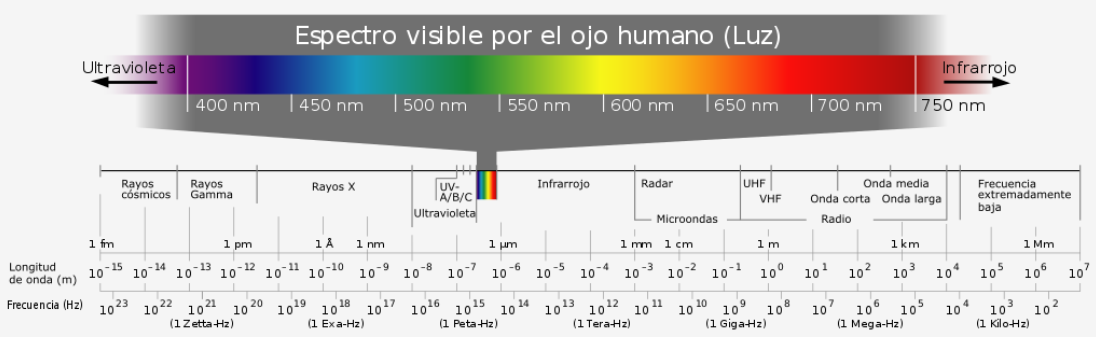
\includegraphics[height=3.8cm]{llumVisible.png}\\\vfill
\end{center}

Aquesta tecnologia utilitza llums fluorescents (làmpades normals, no necessita dispositius especials) per transmetre senyals a una velocitat de 10 kbit/s, o LEDs que pot assolir velocitats de fins a 500 Mbit/s. RONJA aconsegueix assolir una velocitat d'Ethernet completa (10 Mbit/s) sobre la mateixa distància gràcies a una òptica més gran i LED més potents.

La VLC pot ser utilitzada com un mitjà transmissor de computació ubiqua, atès que els dispositius que produeixen llum (làmpades d'interior exterior, televisors, senyals de trànsit, lluminosos comercials, fars de vehicles3) utilitzats a tot arreu, es poden aprofitar. El fer ús de la llum visible és també menys perillosa per a aplicacions que utilitzen una gran potència, ja que, els éssers humans poden percebre i protegirse-se del dany que pugui ocasionar-los.




\subsection*{El mercat del visible Light communication}
\addcontentsline{toc}{subsection}{El mercat del visible Light communication}

\subsubsection*{Visió general del mercat de la Visible Light communication}
Els sistemes de comunicació de llum visible (VLC) s'utilitzen per crear xarxes de comunicació d'alta velocitat, segures i biològicament amigables que permeten la formació i l'expansió d'aplicacions informàtiques unificades. Aquests sistemes utilitzen longituds d'ona de llum modificades emeses per una varietat de fonts, com ara il·luminació exterior i interior, senyals, taulers de visualització, televisors, pantalles d'ordinador, càmeres digitals i càmeres digitals en telèfons mòbils amb finalitats de comunicació, principalment mitjançant l'ús de díodes emissors de llum. (LEDs).

\begin{center}
    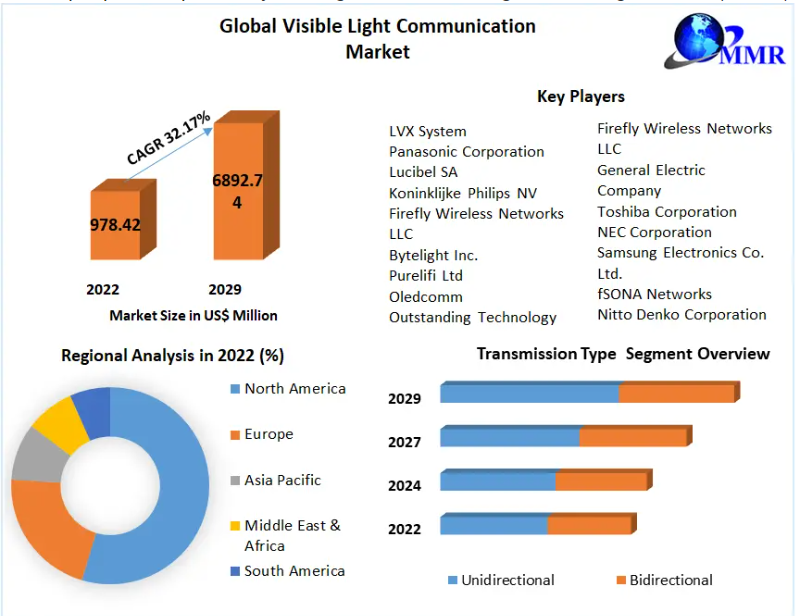
\includegraphics[height=3.8cm]{visiogeneralVLC.png}\\\vfill
\end{center}

La comunicació de llum visible exclourà la necessitat d'altres tecnologies sense fil, com ara infrarojos (IR), Bluetooth i Wi-Fi que emeten interferències electromagnètiques (EMI) i ones de RF que són perjudicials no només per als instruments/dispositius, sinó també per als humans. Així, el mercat es troba en una fase de creixement exponencial i es calcula que creixerà amb un CAGR elevat de xx.xx\% a tot el món durant el període de previsió.

L'estudi de l'informe ha analitzat l'impacte dels ingressos de la pandèmia covid-19 en els ingressos de vendes dels líders del mercat, seguidors del mercat i disruptors a l'informe i el mateix es reflecteix a la nostra anàlisi.




